\documentclass[10pt,spanish,a4paper,openany,notitlepage]{article}
%-------------------------------------Paquetes-----------------------------------------------------------------------
\usepackage[spanish,es-tabla]{babel}  % Traduce los textos a castellano
\usepackage[utf8]{inputenc}	% Permite escribir directamente áéíóúñ
\usepackage{t1enc}      	% Agrega caracteres extendidos al font
\usepackage{amsmath} 	%Permite imprimir mas opcciones matematicas
\usepackage{graphicx}	%Permite agregar imagenes al informe
\usepackage{multicol}  %Permite dividir el texto en varias columnas
\usepackage{float} 	%Permite utilizar H para colocar las imagenes en un lugar especifico 
\usepackage{units}
\usepackage{circuitikz}
\usepackage{caption}
\usepackage{subcaption}
\usepackage{sidecap}
\usepackage{mathtools}
\usepackage{multirow} % Paquete para dividir las tablas en subtablas
\usepackage{booktabs} %estos 2 sirven para achicar la tabla
\usepackage{tabulary}
\usepackage{fancyhdr} % encabezado
\usepackage{textcomp} % para usar ° con el comando \textdegree
\usepackage{anysize}	%Permite modificar los margenes del documento
\usepackage{abstract} % paquete para el resumen del articulo
\usepackage{amssymb}
\usepackage{courier}
\usepackage{color}

\usepackage{etex}     % los 2 siguientes es para poner codigo
\usepackage{listings}


%---------------------------------------Configuraciones de pagina----------------------------------------------
\marginsize{2.5cm}{2.5cm}{1cm}{1cm}

\pagestyle{fancy}
\fancyhf{}
\lhead{
66.17 - \textsc{Sistemas Digitales}\\ 
2\textsuperscript{do} Cuatrimestre de 2015
}
\rhead{
\includegraphics[width=3cm]{imagenes/FIUBA_ALTA.jpg}}
\rfoot{Página \thepage}

%---------------------------------------Definiciones propias---------------------------------------------------------
\newcommand{\oiint}{\displaystyle\bigcirc\!\!\!\!\!\!\!\!\int\!\!\!\!\!\int} %Integral doble cerrada

\DeclarePairedDelimiter\abs{\lvert}{\rvert}%
\DeclarePairedDelimiter\norm{\lVert}{\rVert}%
% Swap the definition of \abs* and \norm*, so that \abs
% and \norm resizes the size of the brackets, and the 
% starred version does not.
\makeatletter
\let\oldabs\abs
\def\abs{\@ifstar{\oldabs}{\oldabs*}}
%
\let\oldnorm\norm
\def\norm{\@ifstar{\oldnorm}{\oldnorm*}}
\makeatother
%--------------------------------------------------------------------------------------------------------------------------------


\makeatletter
\let\ps@plain\ps@fancy 
\makeatother

% lo siguiente es para borrar el titulo del resumen y que no ocupe espacio:
 \AtBeginDocument{%
 \renewcommand{\abstractname}{}%
}
\renewcommand{\absnamepos}{empty} % originally center


\begin{document}

\title{\textbf{TP N\textdegree1: Contador BCD de 4 dígitos con salida a display 7 segmentos}}
\author{
 Vázquez, Matías - 91523\\
 \texttt{mfvazquez@gmail.com}
}
\date{\today}
\maketitle

\begin{abstract} %Resumen
\emph{En el presente Trabajo Práctico se implementará en FPGA un sistema
digital para un contador BCD de 4 dígitos con salida a un display de 
7 segmentos}
\end{abstract}

\section{Especificaciones}

Se implementó en lenguaje descriptor de hardware VHDL un contador BCD de
4 dígitos y un controlador para un display de 7 segmentos de 4 cifras. El
contador se incrementá aproximadamente cada 1 segundo.

Se utilizó el kit de desarrollo ``Spartan-3 Starter Board'' de la empresa
digilent. Utilizando una frecuencia de clock de $50\, \unit{MHz}$.

\subsection{Display de 7 segmentos de 4 cifras}

Cada dígito comparte ocho señales de control para encender cada LED individual
que corresponde a un segmento del carácter. Cada carácter tiene
un ánodo asociado. Poniendo un `0' en el terminal de la FPGA que se 
conecta a ese ánodo, se selecciona el carácter a encenderse.

\begin{figure}[H] %[h] para here [b] para bottom [t] para top [H]+float para aqui si o si
\begin{center}
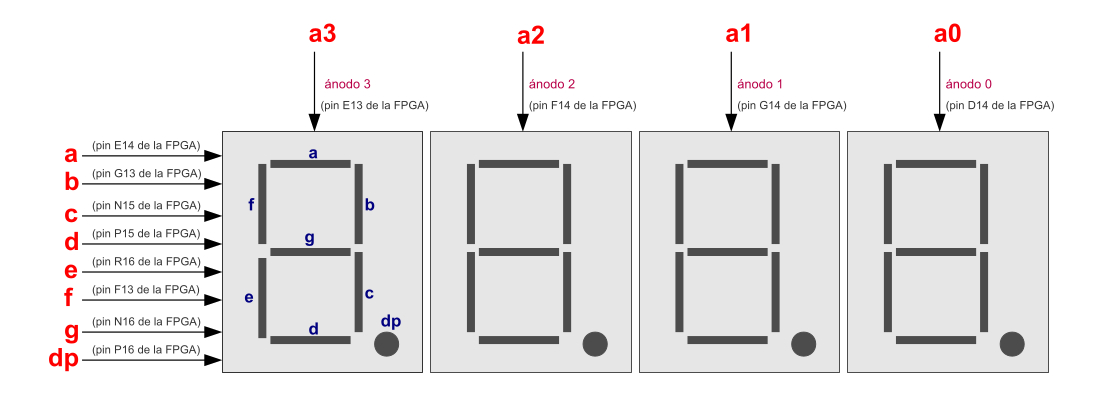
\includegraphics[scale=0.4]{./imagenes/display.png}
\caption{Conexión entre los I/Os de la FPGA y el display}
 \label{fig:display}
\end{center}
\end{figure}

\section{Diseño}

La implementación de cada bloque mostrado en el diagrama en bloques
de la figura \ref{fig:diagrama_bloques} se realizó lo más genérico posible
de forma de poder reutilizar el mismo código a futuro.

\subsection{Diagrama en bloques}

\begin{figure}[H] %[h] para here [b] para bottom [t] para top [H]+float para aqui si o si
\begin{center}
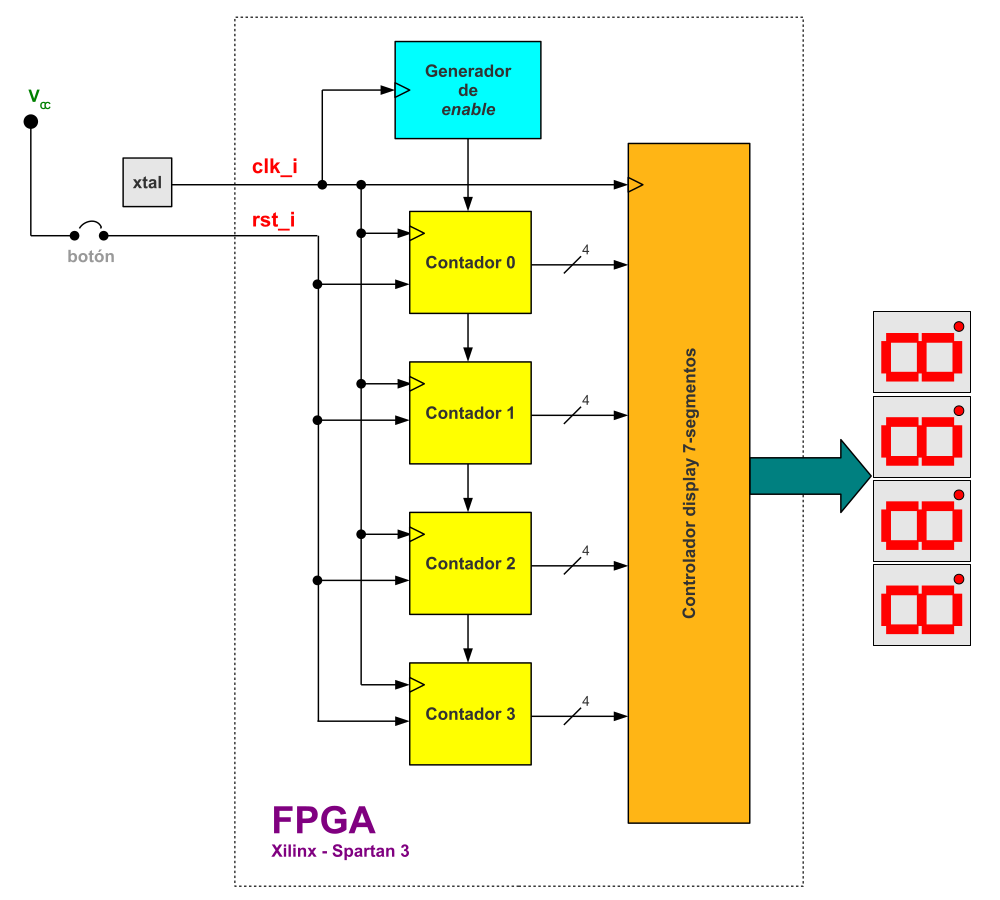
\includegraphics[scale=0.4]{./imagenes/diagrama_bloques.png}
\caption{Diagrama en bloques de la arquitectura}
 \label{fig:diagrama_bloques}
\end{center}
\end{figure}

\subsection{Generador de enable}

Este bloque divide la frecuencia de reloj de la placa a una frecuencia
que tenga un período de aproximadamente $1\, \unit{seg}$.

Para implementarlo se programó un contador de N bits, que devuelve un
1 en su salida durante un período del clock cuando los M bits más 
significativos estén en 1. Pasado este valor se resetea el contador.

Para que cuente aproximadamente $1\, \unit{seg}$ se fijaron los valores
$N = 25$ y $M = 2$. Para así contar hasta que el bit 25 y 24 del contador
estén en 1. El perído de la salida se puede calcular mediante:

\[ \displaystyle T = \frac{2^{25} + 2^{24}}{50\, \unit{MHz}} \approx 1\, \unit{seg} \]

\subsection{Contadores}

Cuentan de 0 a 9, tienen una entrada de reset y una entrada de enable.
Su salida es un contador de 4 bits y 1 bit para el flag de fin de cuenta, 
que solo devolverá 1 si el contador contó hasta 9 y la entrada de enable esta
habilitada.

\subsection{Controlador de display de 7 segmentos}

En la figura \ref{fig:controlador_display} se muestra el diagrama en bloques
de la arquitectura del controlador del display de 7 segmentos.

\begin{figure}[H] %[h] para here [b] para bottom [t] para top [H]+float para aqui si o si
\begin{center}
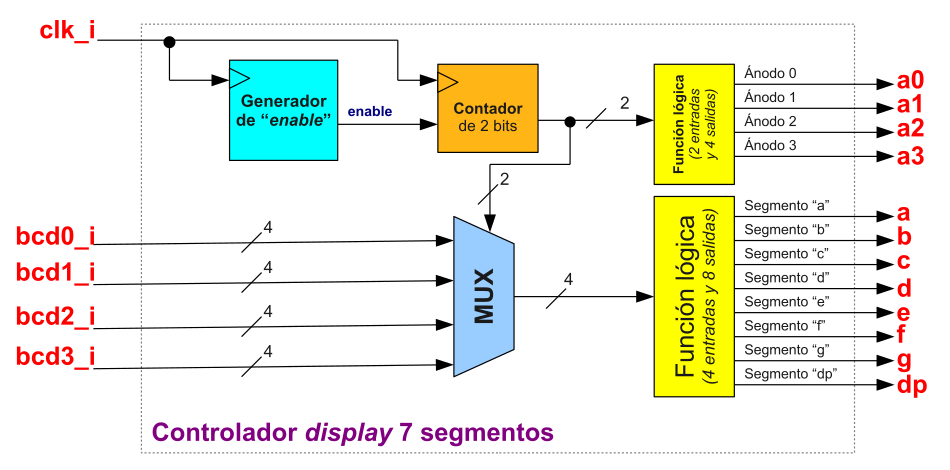
\includegraphics[scale=0.4]{./imagenes/controlador_display.png}
\caption{Arqutectura para el controlador del display de 7 segmentos}
 \label{fig:controlador_display}
\end{center}
\end{figure}

Cuenta con los siguientes elementos:

\begin{itemize}

\item{\bf Multiplexor:} selecciona cuál de las entradas en formato BCD
se imprimirá según lo que indica el contador.

\item{\bf Generador de enable:} Se utilizó el generador de enable genérico
implementado, con $N = 17$ y $M = 21$ de forma que cada cifra del display
se encienda aproximadamente a una frecuencia de $100\, \unit{Hz}$. Como
son 4 cifras, deberá devolver una salida con una frecuencia de $400\, \unit{Hz}$
aproximadamente. Por lo que la frecuencia de salida se la puede calcular mediante:

\[ \displaystyle f = \frac{50\, \unit{MHz}}{2^{17}} \approx 381,5\, \unit{Hz} \]

\item{\bf Función lógica de 4 entradas y 8 salidas:} Es la encargada
de mapear los números en formato BCD a los LEDs que deben encenderse para
representar dicho número.

\item{\bf Función lógica de 2 entradas y 4 salidas:} Es la encargada
de seleccionar el ánodo según el valor del contador

\item{\bf Contador de 2 bits:} Es el encargado de conmutar el ánodo para mantener 
las 4 cifras del display encendidas. Para hacerlo lo más genérico posible
se implementó un contador de N bits, que cuenta hasta que todos sus
bits sean 1.

\end{itemize}

\section{Simulaciones}

A continuación se muestran algunas simulaciones realizadas mediante pruebas.

\subsection{Contador}

\begin{figure}[H] %[h] para here [b] para bottom [t] para top [H]+float para aqui si o si
\begin{center}
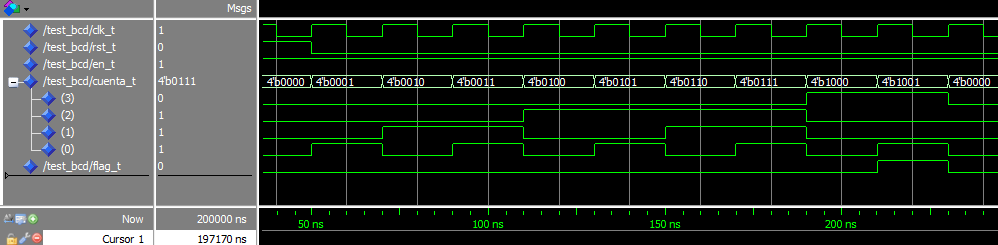
\includegraphics[scale=0.6]{./imagenes/BCD.png}
\caption{Simulación de BCD\_test.vhd}
 \label{fig:sim_BCD}
\end{center}
\end{figure}

\subsection{Contador de N bits}

Para esta prueba se utilizó $N = 4$, que es la cantidad de bits del contador.

\begin{figure}[H] %[h] para here [b] para bottom [t] para top [H]+float para aqui si o si
\begin{center}
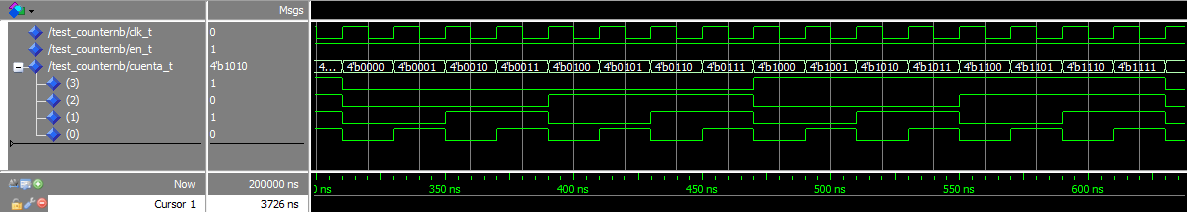
\includegraphics[scale=0.5]{./imagenes/ContadorNb.png}
\caption{Simulación de CounterNb\_test.vhd}
 \label{fig:sim_ContadorNb}
\end{center}
\end{figure}

\subsection{Multiplexor}

Para esta prueba las entradas del multiplexor eran: $1000$, $0100$, $0010$ y $0001$.

\begin{figure}[H] %[h] para here [b] para bottom [t] para top [H]+float para aqui si o si
\begin{center}
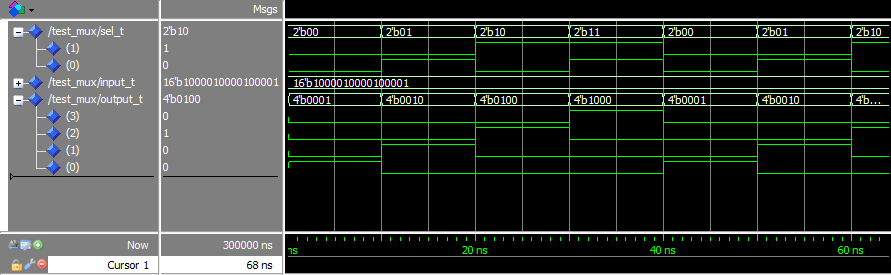
\includegraphics[scale=0.6]{./imagenes/Mux.png}
\caption{Simulación de Mux\_test.vhd}
 \label{fig:sim_Mux}
\end{center}
\end{figure}

\subsection{Selector de display}

\begin{figure}[H] %[h] para here [b] para bottom [t] para top [H]+float para aqui si o si
\begin{center}
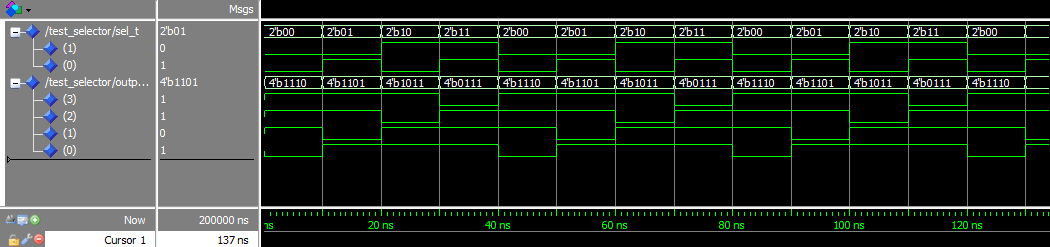
\includegraphics[scale=0.6]{./imagenes/selector.png}
\caption{Simulación de Selector\_test.vhd}
 \label{fig:sim_Selector}
\end{center}
\end{figure}

\subsection{Contador BCD de 4 digitos con salida a display de 7 segmentos}

\begin{figure}[H] %[h] para here [b] para bottom [t] para top [H]+float para aqui si o si
\begin{center}
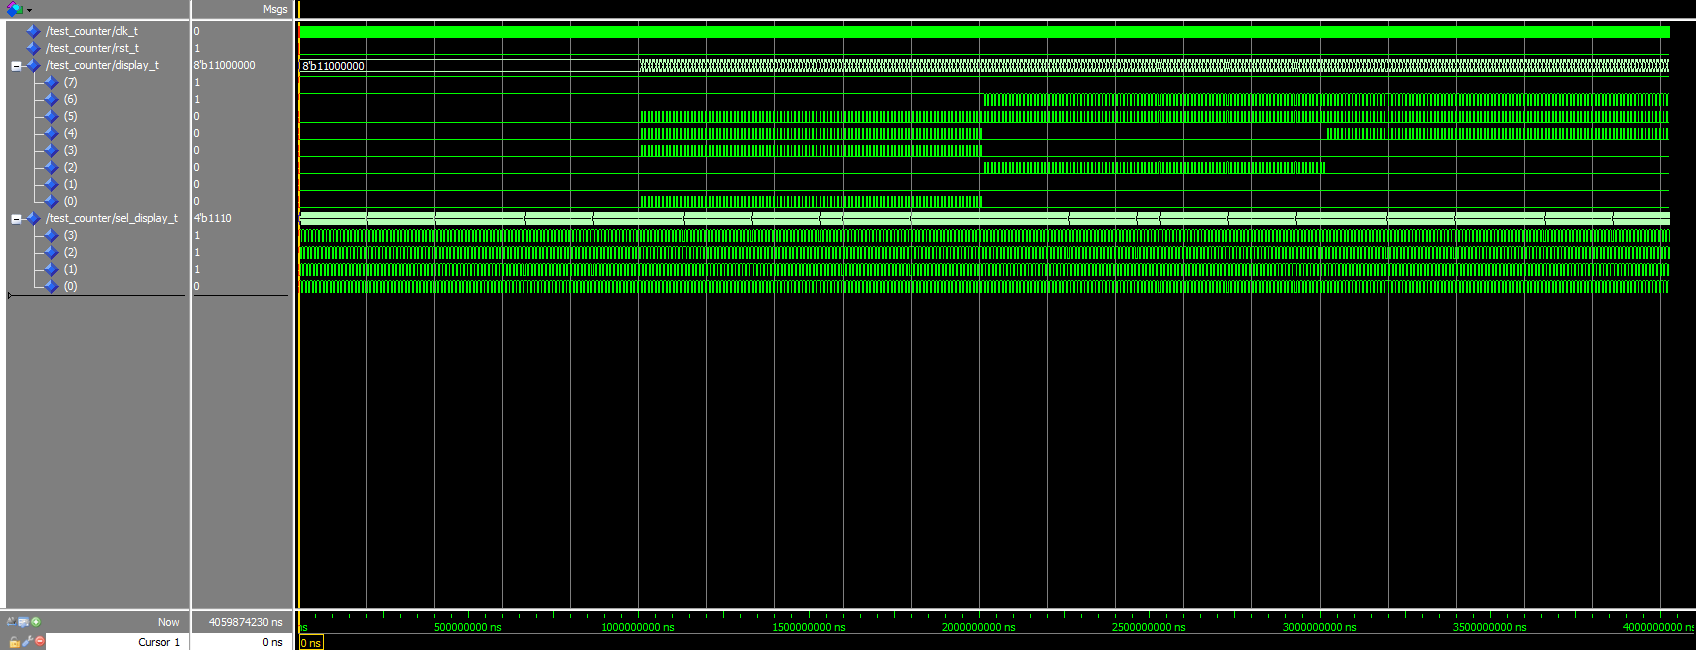
\includegraphics[scale=0.4]{./imagenes/Counter.png}
\caption{Simulación de Counter\_test.vhd}
 \label{fig:sim_Counter}
\end{center}
\end{figure}


\section{Resumen de síntesis}

\begin{center}
\begin{tabular}{|c|c|c|}\hline
Utilización Lógica & Usados & Utilización \\\hline
Slices & $69$ & $3\, \unit{\%}$ \\\hline
Flip-Flops & $68$ & $1\, \unit{\%}$ \\\hline
LUTs & $138$ & $3\, \unit{\%}$ \\\hline
GCLK  & $1$ & $12\, \unit{\%}$ \\\hline\hline
frecuencia máxima &  \multicolumn{2}{c|}{$119.147\, \unit{MHz}$} \\\hline
\end{tabular}
\end{center}

\newpage
\section{Código fuente VHDL}

\subsection{GenEna.vhd}
\lstinputlisting[language=VHDL]{../codigo/GenEna.vhd}
\newpage

\subsection{GenEna\_test.vhd}
\lstinputlisting[language=VHDL]{../codigo/GenEna_test.vhd}
\newpage

\subsection{BCD.vhd}
\lstinputlisting[language=VHDL]{../codigo/BCD.vhd}
\newpage

\subsection{BCD\_test.vhd}
\lstinputlisting[language=VHDL]{../codigo/BCD_test.vhd}
\newpage

\subsection{BCD4\_test.vhd}
\lstinputlisting[language=VHDL]{../codigo/BCD4_test.vhd}
\newpage

\subsection{Mux.vhd}
\lstinputlisting[language=VHDL]{../codigo/Mux.vhd}
\newpage

\subsection{Mux\_test.vhd}
\lstinputlisting[language=VHDL]{../codigo/Mux_test.vhd}
\newpage


\subsection{Serializer.vhd}
\lstinputlisting[language=VHDL]{../codigo/Serializer.vhd}
\newpage

\subsection{Serializer\_test.vhd}
\lstinputlisting[language=VHDL]{../codigo/Serializer_test.vhd}
\newpage

\subsection{Selector.vhd}
\lstinputlisting[language=VHDL]{../codigo/Selector.vhd}
\newpage

\subsection{Selector\_test.vhd}
\lstinputlisting[language=VHDL]{../codigo/Selector_test.vhd}
\newpage



\subsection{CounterNb.vhd}
\lstinputlisting[language=VHDL]{../codigo/CounterNb.vhd}
\newpage

\subsection{CounterNb\_test.vhd}
\lstinputlisting[language=VHDL]{../codigo/CounterNb_test.vhd}
\newpage



\subsection{DisplayController.vhd}
\lstinputlisting[language=VHDL]{../codigo/DisplayController.vhd}
\newpage

\subsection{DisplayController\_test.vhd}
\lstinputlisting[language=VHDL]{../codigo/DisplayController_test.vhd}
\newpage



\subsection{Counter.vhd}
\lstinputlisting[language=VHDL]{../codigo/Counter.vhd}
\newpage



\subsection{Counter\_test.vhd}
\lstinputlisting[language=VHDL]{../codigo/Counter_test.vhd}
\newpage



\end{document}
